[9~v\textsuperscript{o}] Nec refert dicere in circulo ob latera polygoni ejus infinite parva, etiam elevationem\protect\index{Sachverzeichnis}{elevatio} fore infinite parvam, ac proinde contemnendam: nam etsi latera sint infinite parva, sunt tamen infinita multitudine. At vero infinite parvum infinities \edtext{repetitum, quantitatem}{\lemma{repetitum,}\Bfootnote{\textit{(1)}\ rem \textit{(2)}\ quantitatem \textit{L}}} componit finite parvam, sive ordinariam, neque contemnendam.% \\
\pend
\count\Cfootins=1500
\count\Bfootins=1200
\pstart 
\vspace{1.5em}
\noindent
[\textit{Zeichnungen \setline{1}am unteren Rand von Bl. 9~r\textsuperscript{o}:}] 
\pend
\vspace{1em}
\pstart \noindent
\begin{minipage}[b] {0.5\textwidth}
 \includegraphics[trim = 0mm 0mm 0mm 0mm, clip, width=0.8\textwidth]{images/lh03705_009r-d4.pdf}
 \vspace{4mm}
\end{minipage}
%\hspace*{13,3mm}
\begin{minipage}[b] {0.5\textwidth}
\includegraphics[trim = 0mm 0mm 0mm 0mm, clip, width=1.0\textwidth]{images/lh03705_009r-d5.pdf}
\end{minipage}
\pend
\vspace{0.3em}
\pstart
\hspace{10mm}\setline{1}  [\textit{Fig. 12}] \hspace{60mm} [\textit{Fig. 13}]
\pend
\vspace{1em}
\pstart                                
  \noindent \centering 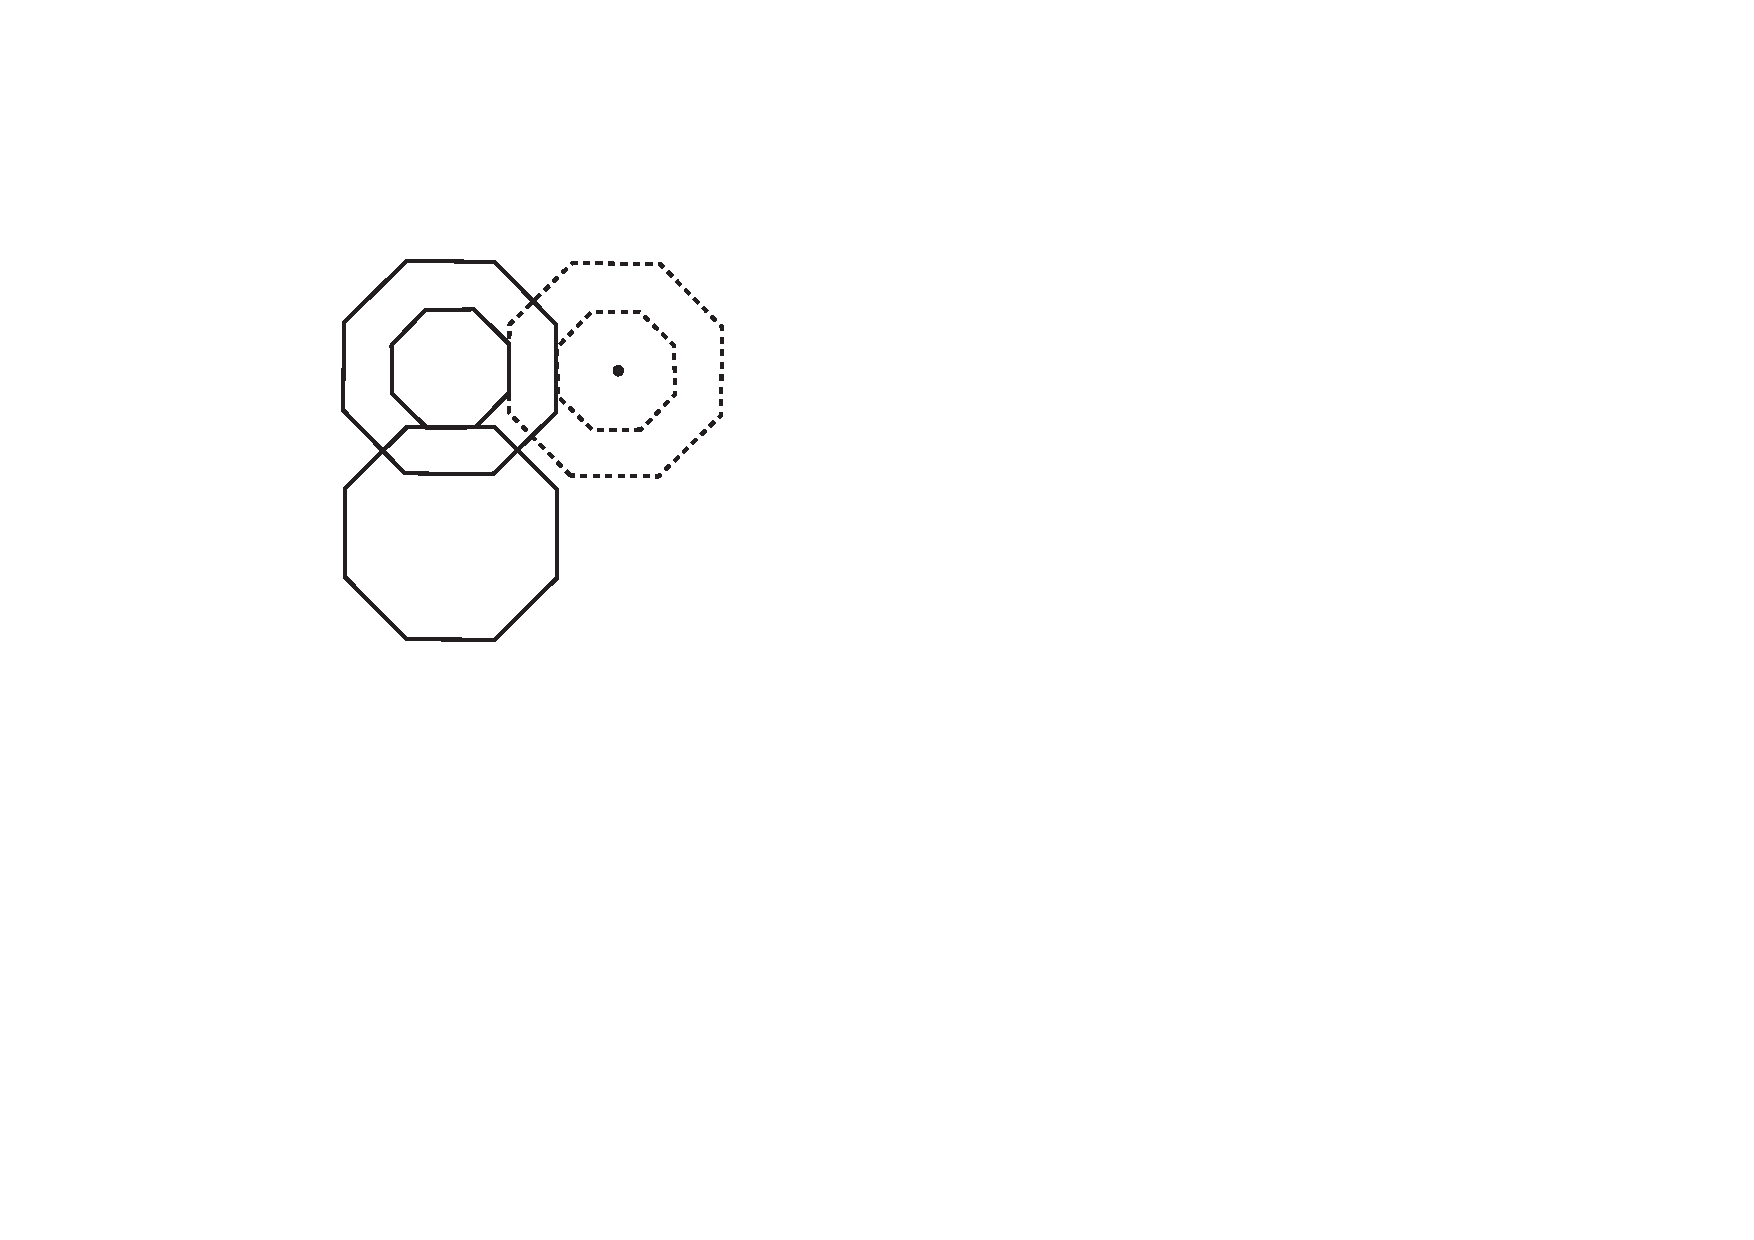
\includegraphics[trim = 0mm -4mm 0mm 0mm, clip, width=0.27\textwidth]{images/lh03705_009r-d6.pdf}\\
\centering [\textit{Fig. 14}]
\pend
\newpage
\pstart 
%\vspace{8mm}
%    \begin{wrapfigure}{l}{0.4\textwidth}
\noindent  \centering 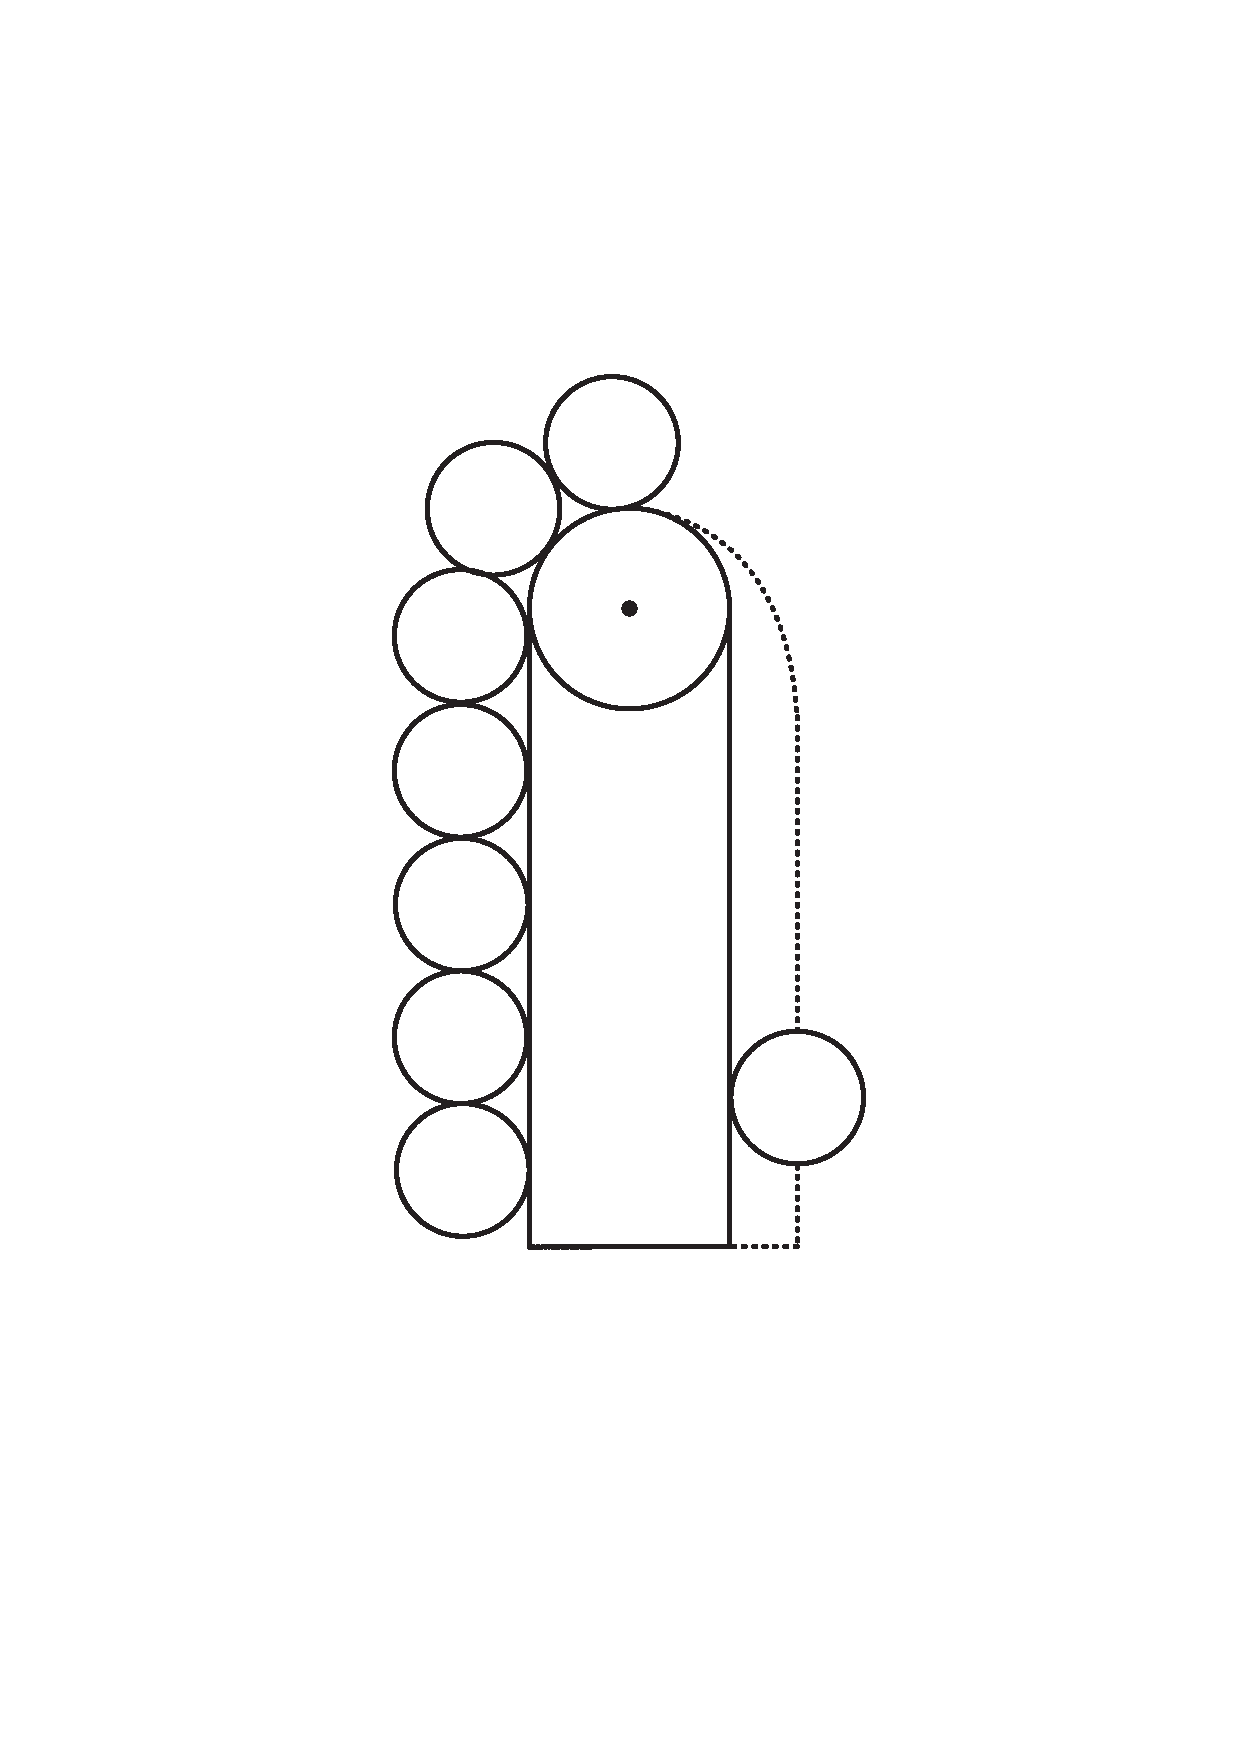
\includegraphics[trim = 0mm -5mm 0mm 0mm, clip,width=0.2\textwidth]{images/lh03705_009v-d1.pdf}
\pend
\pstart
 % \vspace*{4mm}
%    \caption{Bildbeschreibung}
%    \end{wrapfigure}
 \noindent
[\edtext{\textit{Fig. 15, gestrichene Zeichnung}}{\lemma{\hspace{1.8mm}[\textit{Fig. 15}]}\killnumber\Cfootnote{Ähnliche Zeichnungen finden sich in N.~9, N.~18 und N.~95.}} \textit{ohne erkennbaren Zusammenhang mit dem Text, urspr\"{u}ng\-lich auf Bl. 8~r\textsuperscript{o}:}] 
\pend
\count\Cfootins=1500
\count\Bfootins=1500
